\documentclass{article}
\usepackage{tikz}
\usetikzlibrary{matrix}

\begin{document}

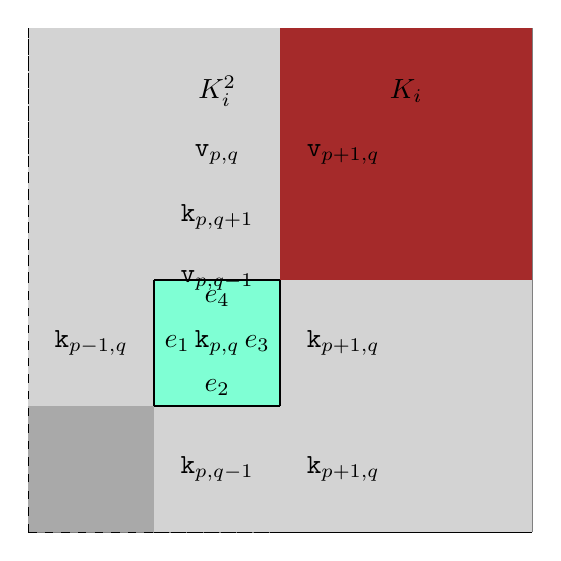
\begin{tikzpicture}[scale=0.8]
    % Define colors
    \definecolor{lightgray}{RGB}{211,211,211}
    \definecolor{darkgray}{RGB}{169,169,169}
    \definecolor{bluegray}{RGB}{139,139,139}
    \definecolor{cyan}{RGB}{127,255,212}
    \definecolor{brown}{RGB}{165,42,42}

    % Draw the grid
    \draw[help lines] (0,0) grid (8,8);

    % Draw the shaded regions
    \fill[lightgray] (0,0) rectangle (8,8);
    \fill[darkgray] (0,0) rectangle (2,2);
    \fill[cyan] (2,2) rectangle (4,4);
    \fill[brown] (4,4) rectangle (8,8);

    % Draw the vertical dashed line
    \draw[dashed] (0,0) -- (0,8);
    \draw[dashed] (0,4) -- (0,8);
    \draw[dashed] (0,6) -- (0,8);

    % Draw the horizontal dashed line
    \draw[dashed] (0,0) -- (8,0);
    \draw[dashed] (2,0) -- (8,0);
    \draw[dashed] (4,0) -- (8,0);
    \draw[dashed] (6,0) -- (8,0);

    % Draw the fine element with edges
    \fill[cyan] (2,2) rectangle (4,4);
    \draw[thick] (2,2) -- (2,4) node[midway, right] {$e_1$};
    \draw[thick] (2,2) -- (4,2) node[midway, above] {$e_2$};
    \draw[thick] (4,2) -- (4,4) node[midway, left] {$e_3$};
    \draw[thick] (2,4) -- (4,4) node[midway, below] {$e_4$};

    % Label the elements
    \node at (3,3) {$\mathtt{k}_{p,q}$};
    \node at (3,5) {$\mathtt{k}_{p,q+1}$};
    \node at (1,3) {$\mathtt{k}_{p-1,q}$};
    \node at (5,3) {$\mathtt{k}_{p+1,q}$};
    \node at (3,1) {$\mathtt{k}_{p,q-1}$};
    \node at (5,1) {$\mathtt{k}_{p+1,q}$};
    \node at (3,7) {$K_i^2$};
    \node at (6,7) {$K_i$};
    \node at (3,6) {$\mathtt{v}_{p,q}$};
    \node at (5,6) {$\mathtt{v}_{p+1,q}$};
    \node at (3,4) {$\mathtt{v}_{p,q-1}$};
\end{tikzpicture}

\end{document}